% A poster using beamerposter and the gemini theme with epfl colors.
% Beamerposter will let you create a poster in a single beamer frame
% using the columns and blocks from the beamer class.
% The color theme is adapted from Gemini's MIT scheme.

% use beamer as documentclass
\documentclass[final]{beamer}

% use the beamerposter package to create a poster
\usepackage[scale=1.4,orientation=portrait,size=a0]{beamerposter}
\usepackage{csquotes}
\usepackage[backend=biber,giveninits=true,maxbibnames=99,bibencoding=utf8,style=numeric]{biblatex}
\addbibresource{references.bib}
% make references small
\renewcommand*{\bibfont}{\scriptsize}

% use the gemini theme.
\usetheme{gemini}
% use the epfl color theme, defining:
% - epflred / rouge
% - epfldarkred / groseille
% - epflgreen / leman
% - epfldarkgreen / canard
% - epflgray / perle
% - epfldark / ardoise
% - epfllight (not official, but included for very light backgrounds)

\usecolortheme{epfl}

\usepackage{graphicx}
\usepackage{tikz}
\usepackage{adjustbox}
\usepackage{qrcode}
\usepackage{wrapfig}
\usepackage{blindtext}
\usepackage{subcaption}
\usepackage{fontawesome}

\title{Inferring Tonality from Note Distributions: \\ Why Models Matter}

\author{Fabian C. Moss and Martin Rohrmeier}

\institute{Digital and Cognitive Musicology Lab, École Polytechnique Fédérale de Lausanne}


\begin{document}

\begin{frame}[t]

  \begin{minipage}[t][.65\textheight][t]{\textwidth}

  \begin{columns}[t]
    \begin{column}{0.3\textwidth}
      \begin{block}{Background}
        \alert{Pitch-class statistics} in pieces correspond to \alert{cognitive representations} of tonality \cite{Albrecht2013,Harasim2019,Krumhansl1982, Temperley2001} and assumed to constitute the basis for statistical learning.

        \begin{figure}
          \centering
          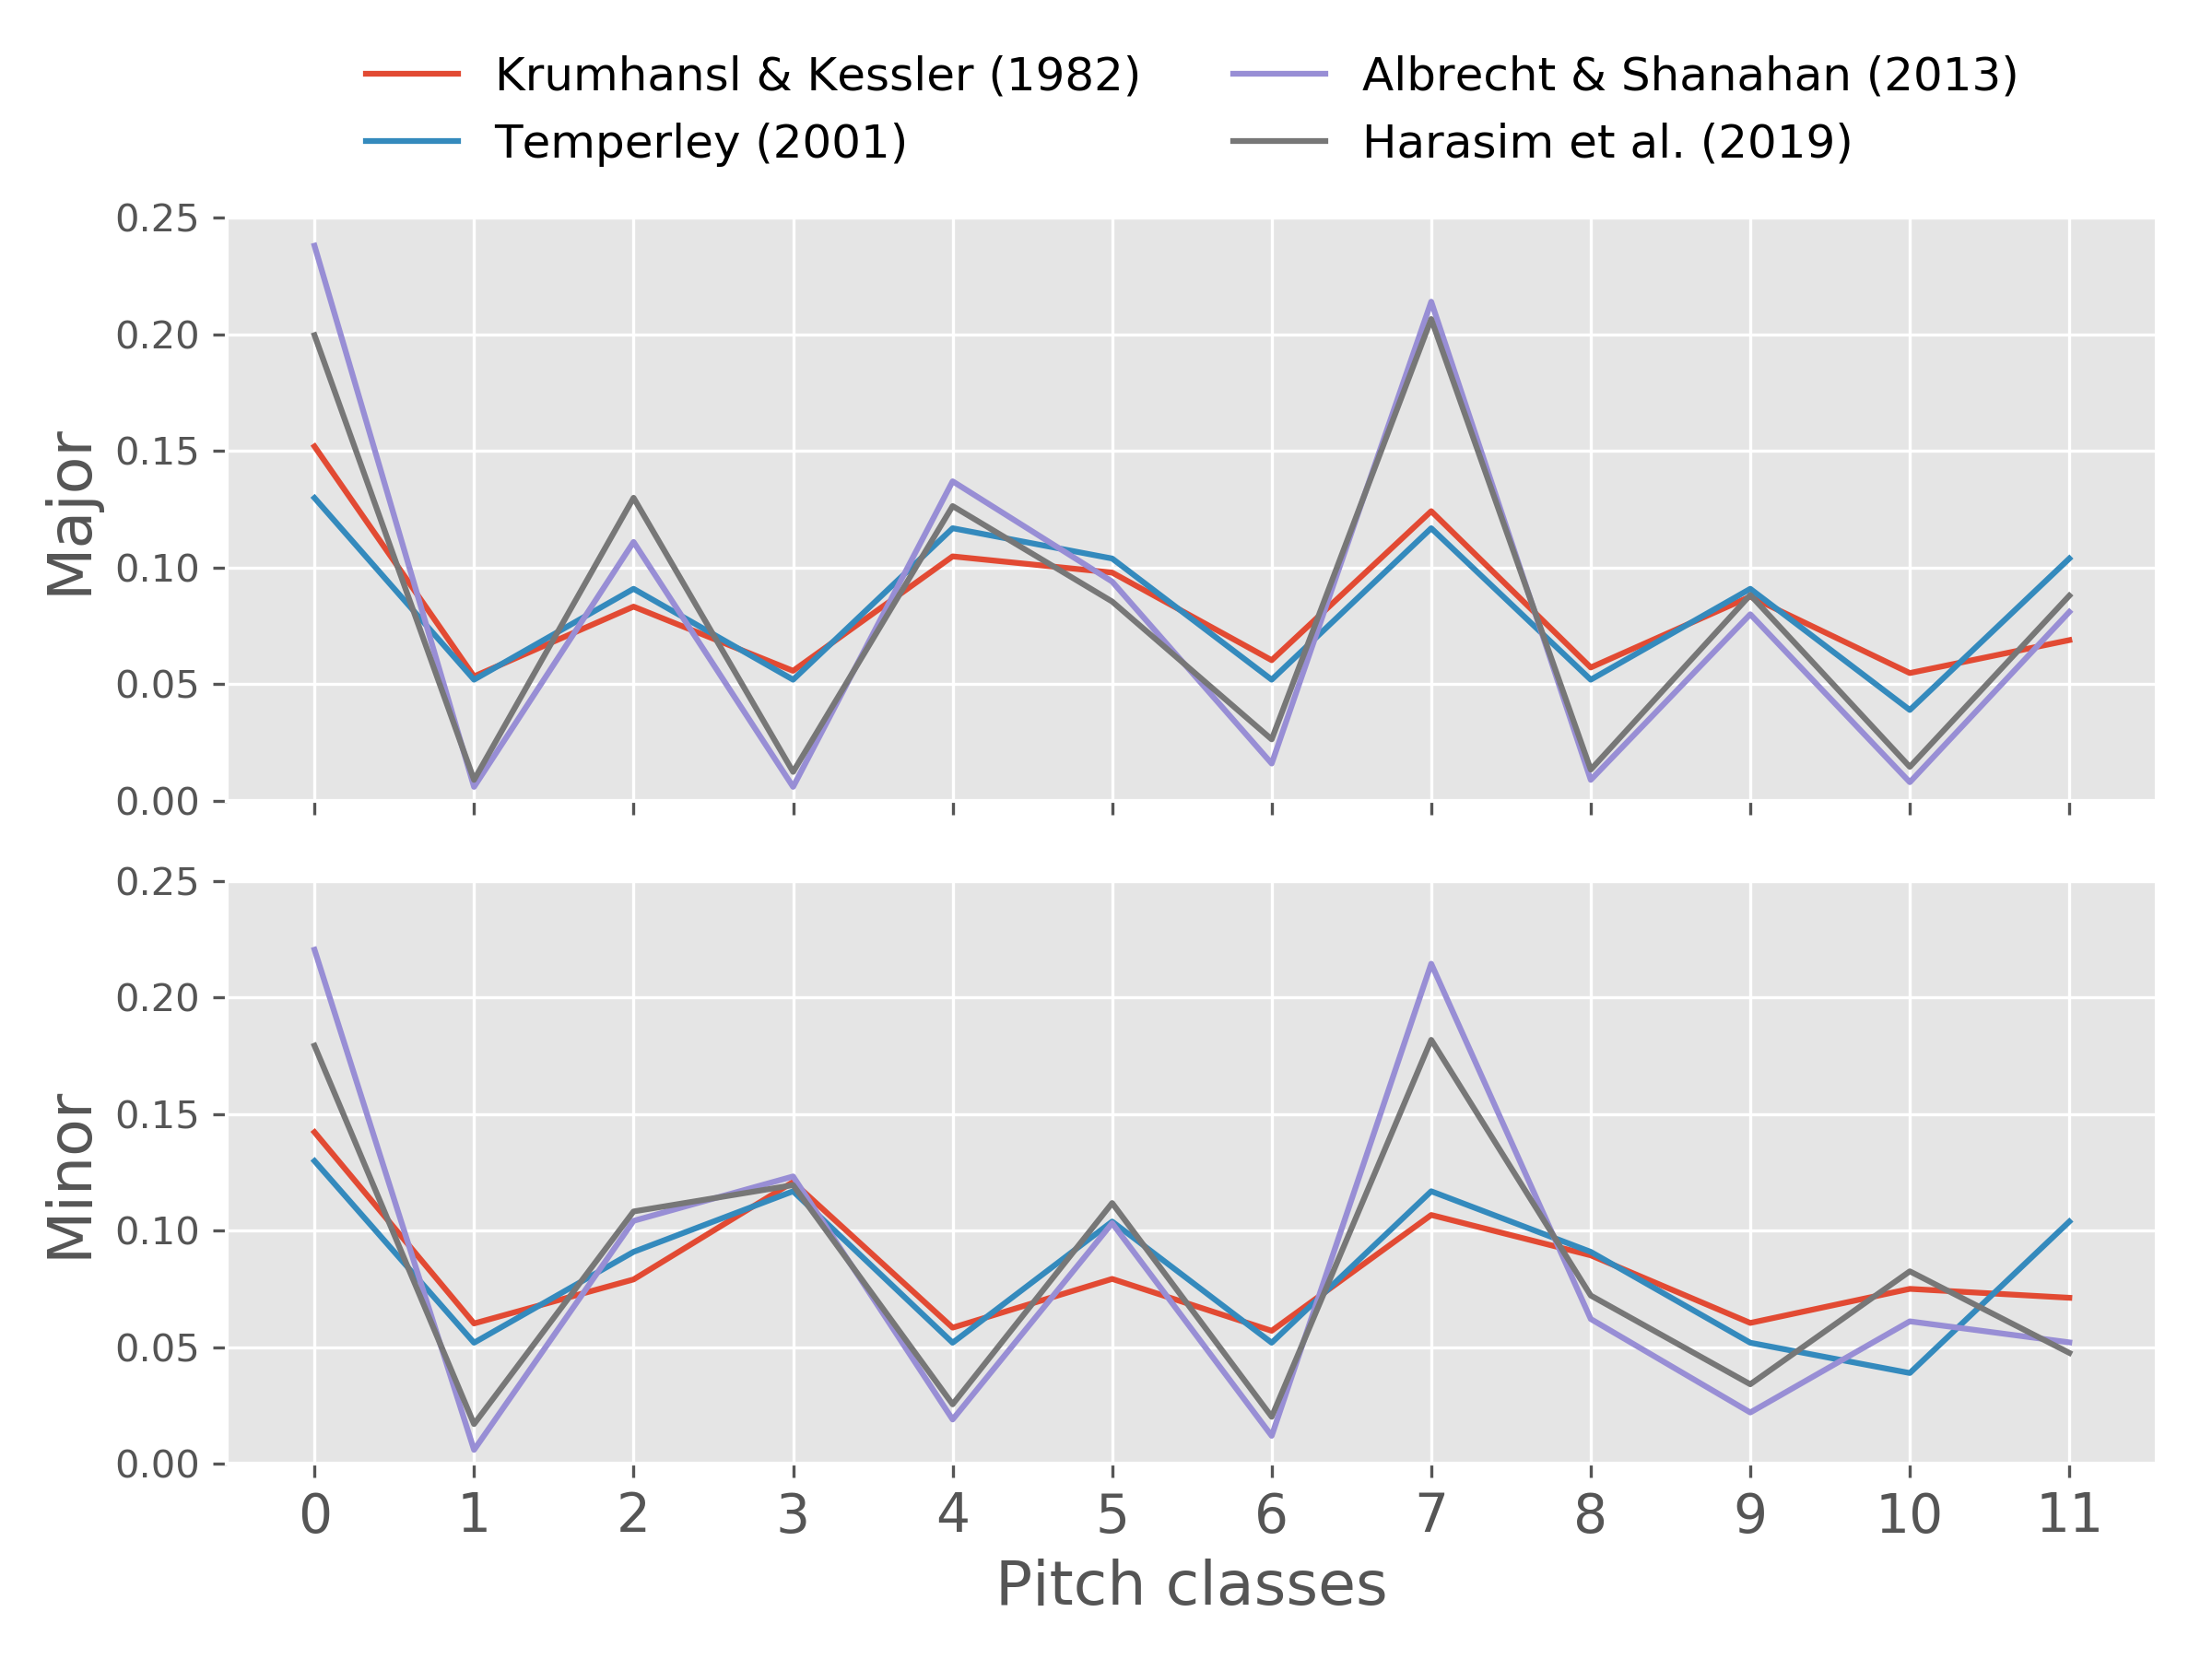
\includegraphics[width=\textwidth]{img/templates}
        \end{figure}
      \end{block}

      \begin{block}{Model 1: Circle of Fifths}
				\alert{Reordering} pitch classes by $x\mapsto 7x \mod 12$ and arranging them on the \alert{circle of fifths} emphasizes differences and similarities of the major and the minor mode \autocite{Harasim2019}. \textbf{IMPORTANCE OF THE FIFTH}
        \begin{figure}
          \centering
          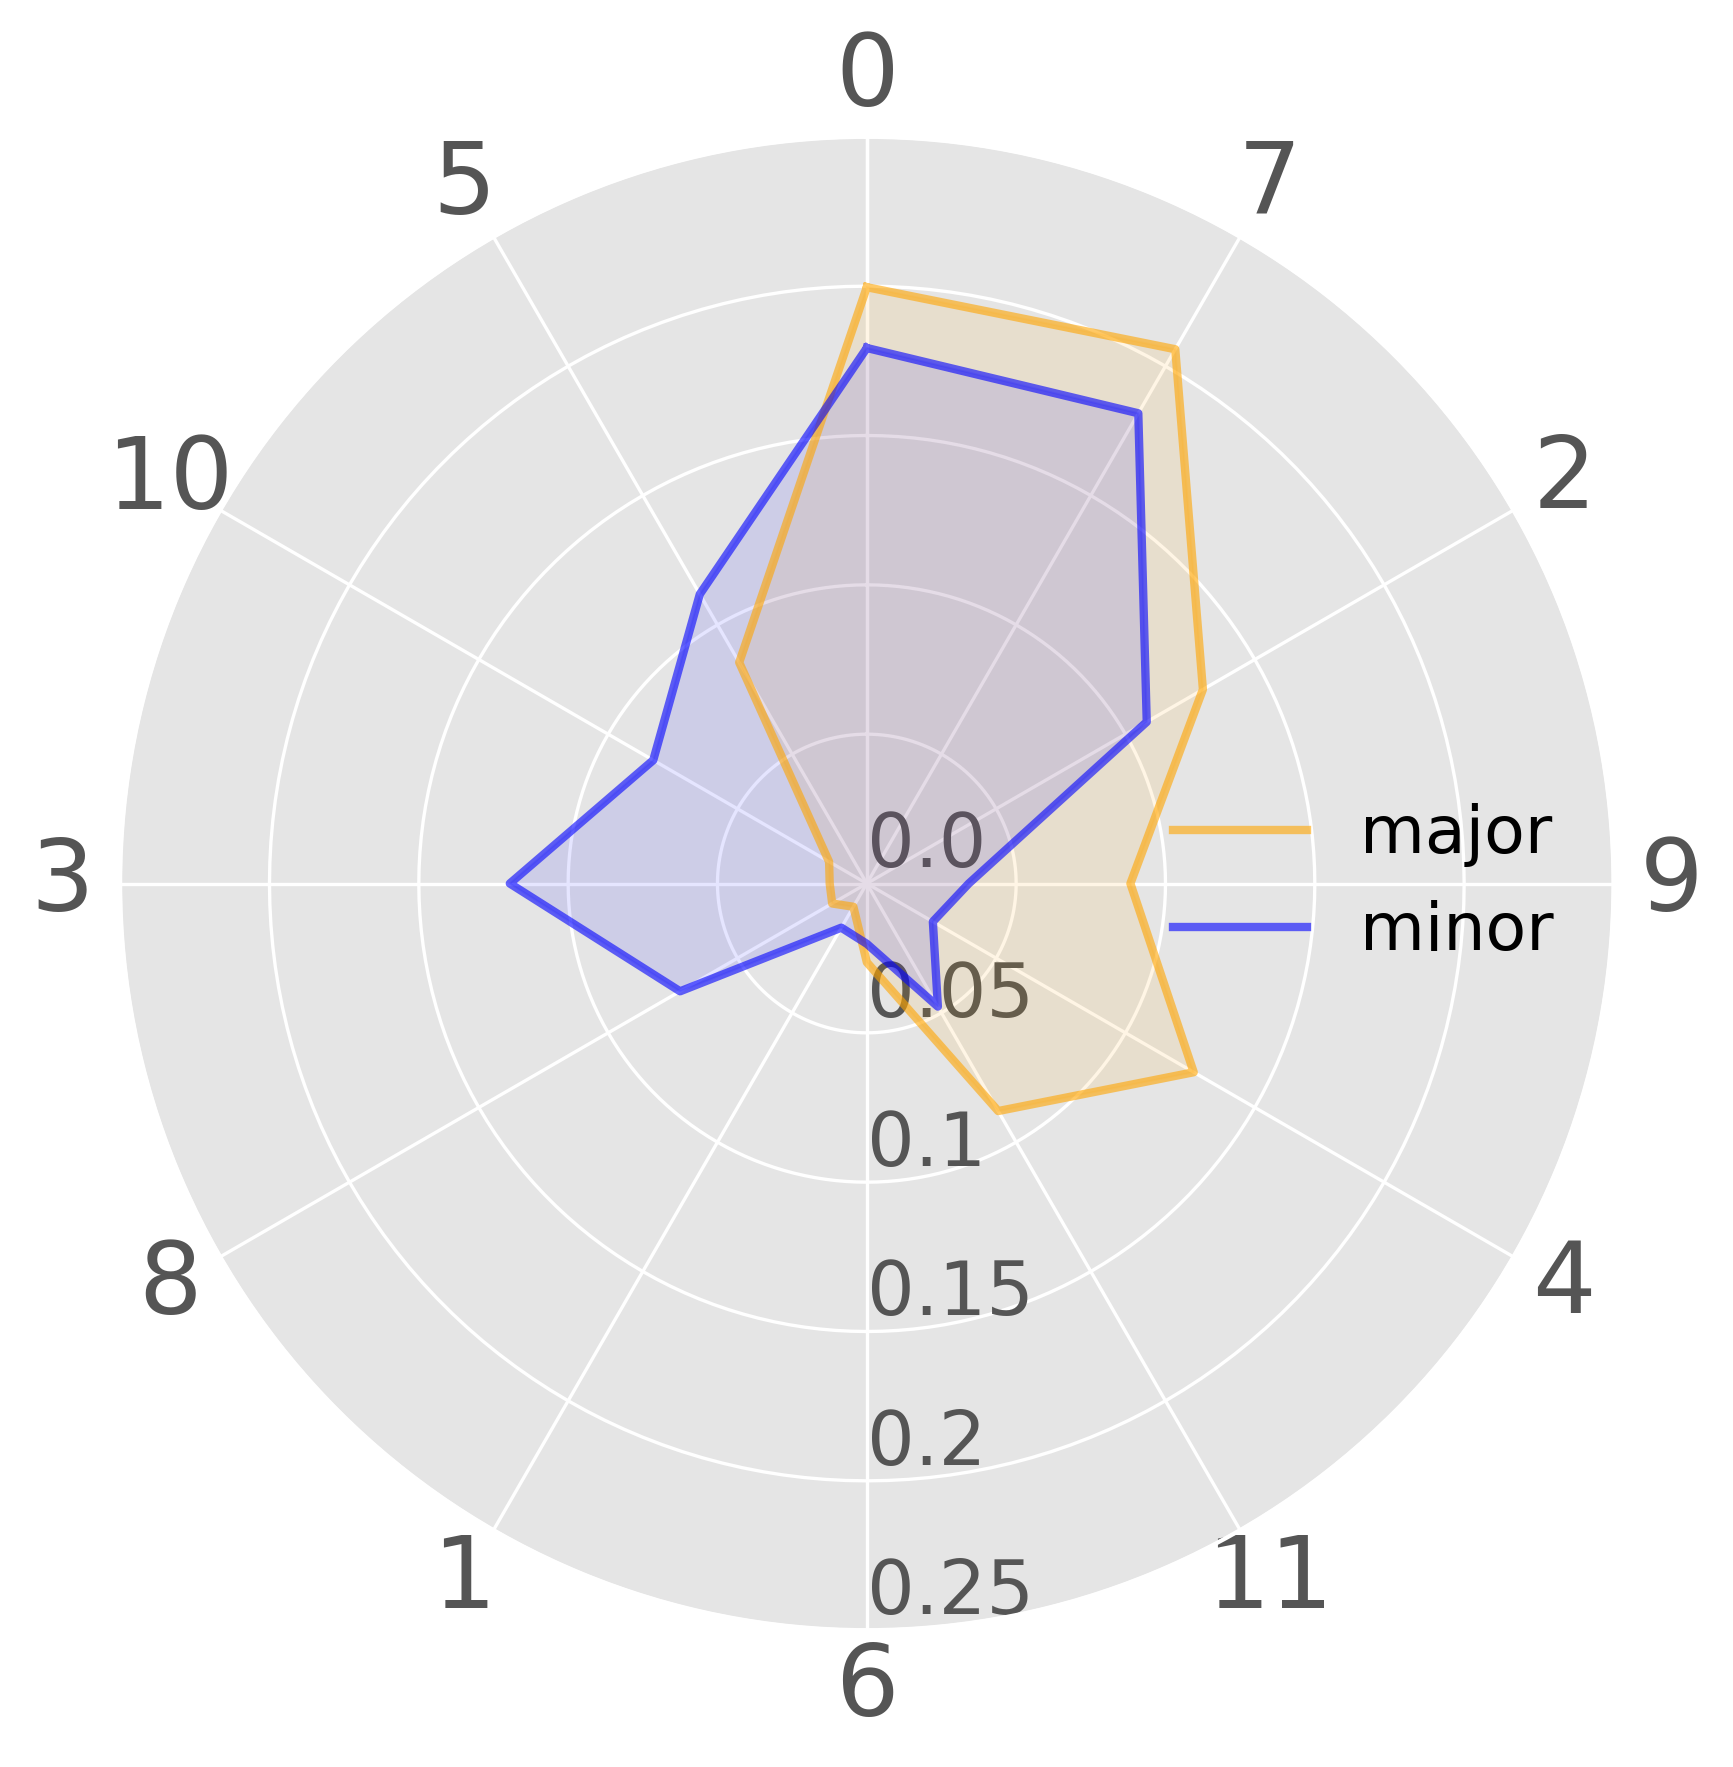
\includegraphics[width=.85\textwidth]{img/radars}
        \end{figure}
      \end{block}

    \end{column}

    \begin{column}{0.3\textwidth}

      \begin{block}{Model 2: Line of Fifths}
        Using \alert{spelled pitch classes} enables the distinction between diatonic, chromatic, and enharmonic pieces \autocite{Gardonyi2002} and indicates a historical trend towards expansion of the tonal material (see "Historical Development") \textbf{EXPANSION IN FIFTH-DIRECTION}.
        \begin{figure}
				\centering

				\begin{subfigure}{\textwidth} % width of left subfigure
					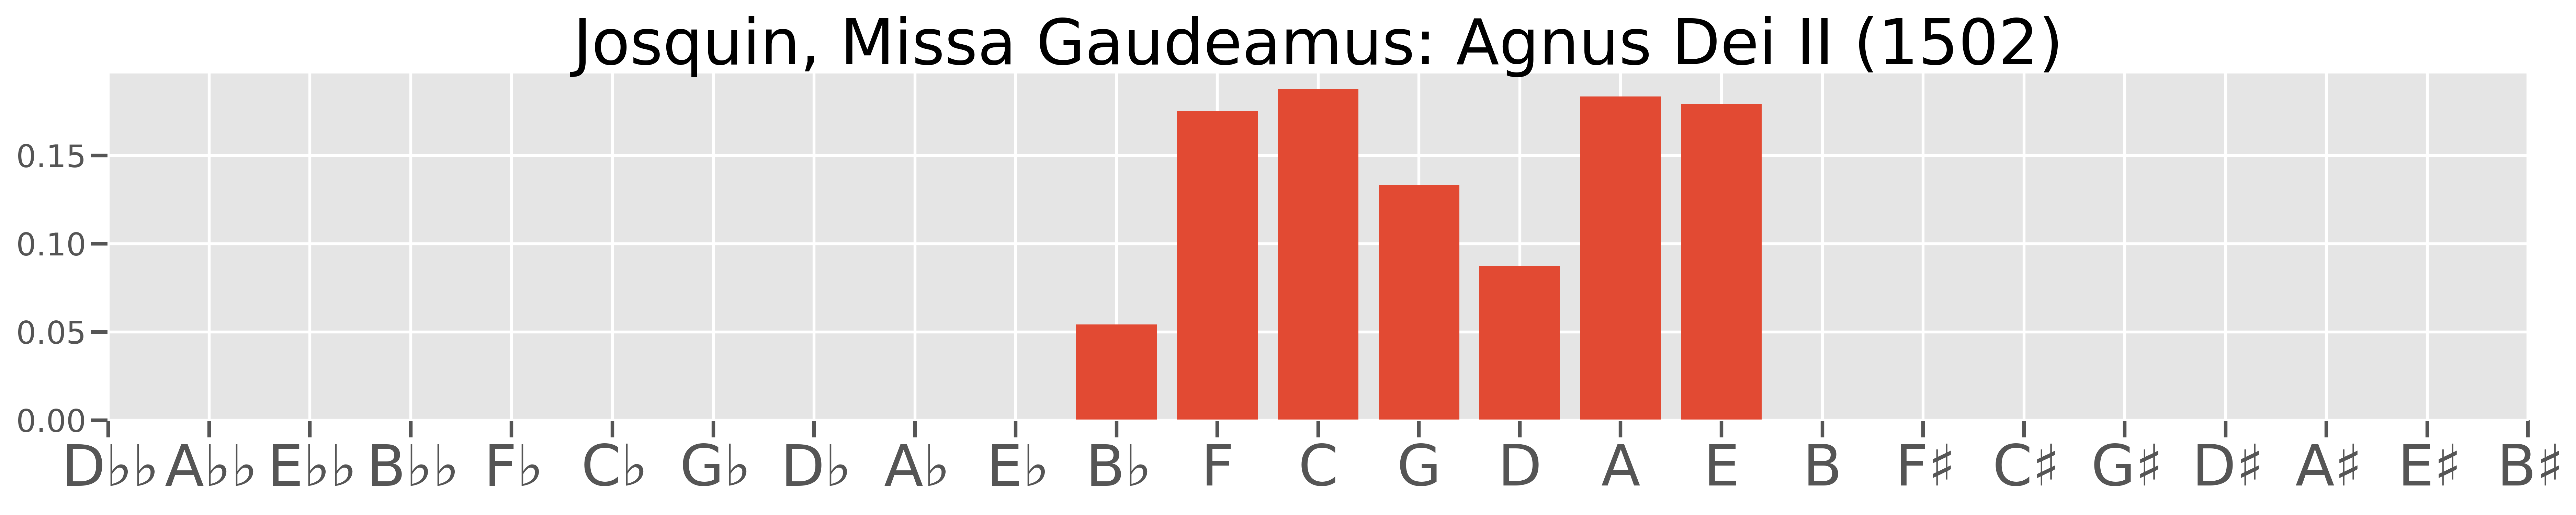
\includegraphics[width=\textwidth]{img/gmm_josquin.png}
				\end{subfigure}

				\vspace{1em} % here you can insert horizontal or vertical space

				\begin{subfigure}{\textwidth} % width of left subfigure
					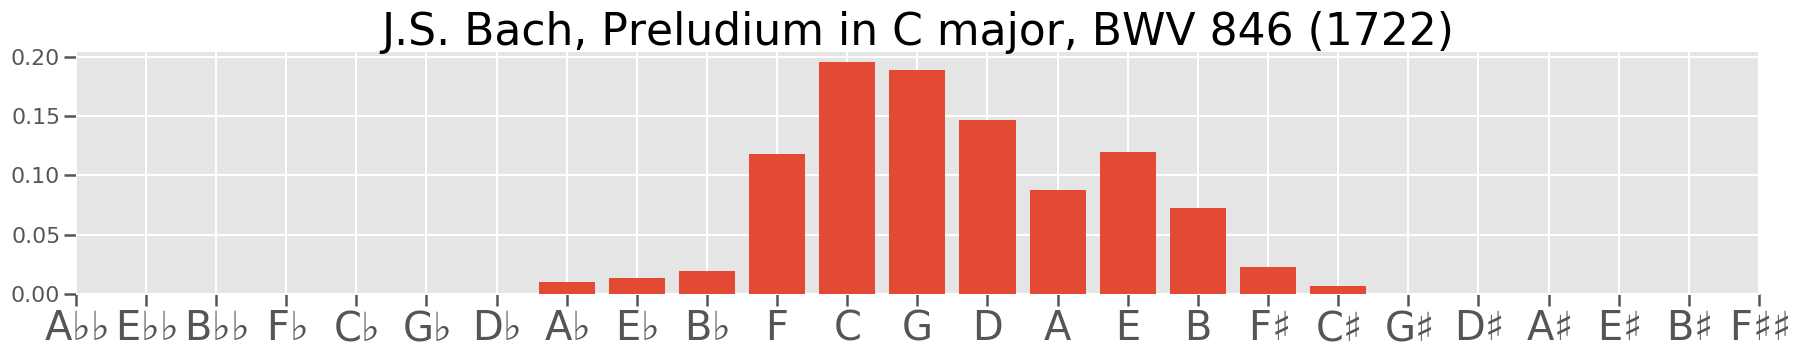
\includegraphics[width=\textwidth]{img/gmm_bach.png}
				\end{subfigure}

				\vspace{1em} % here you can insert horizontal or vertical space

				\begin{subfigure}{\textwidth} % width of right subfigure
					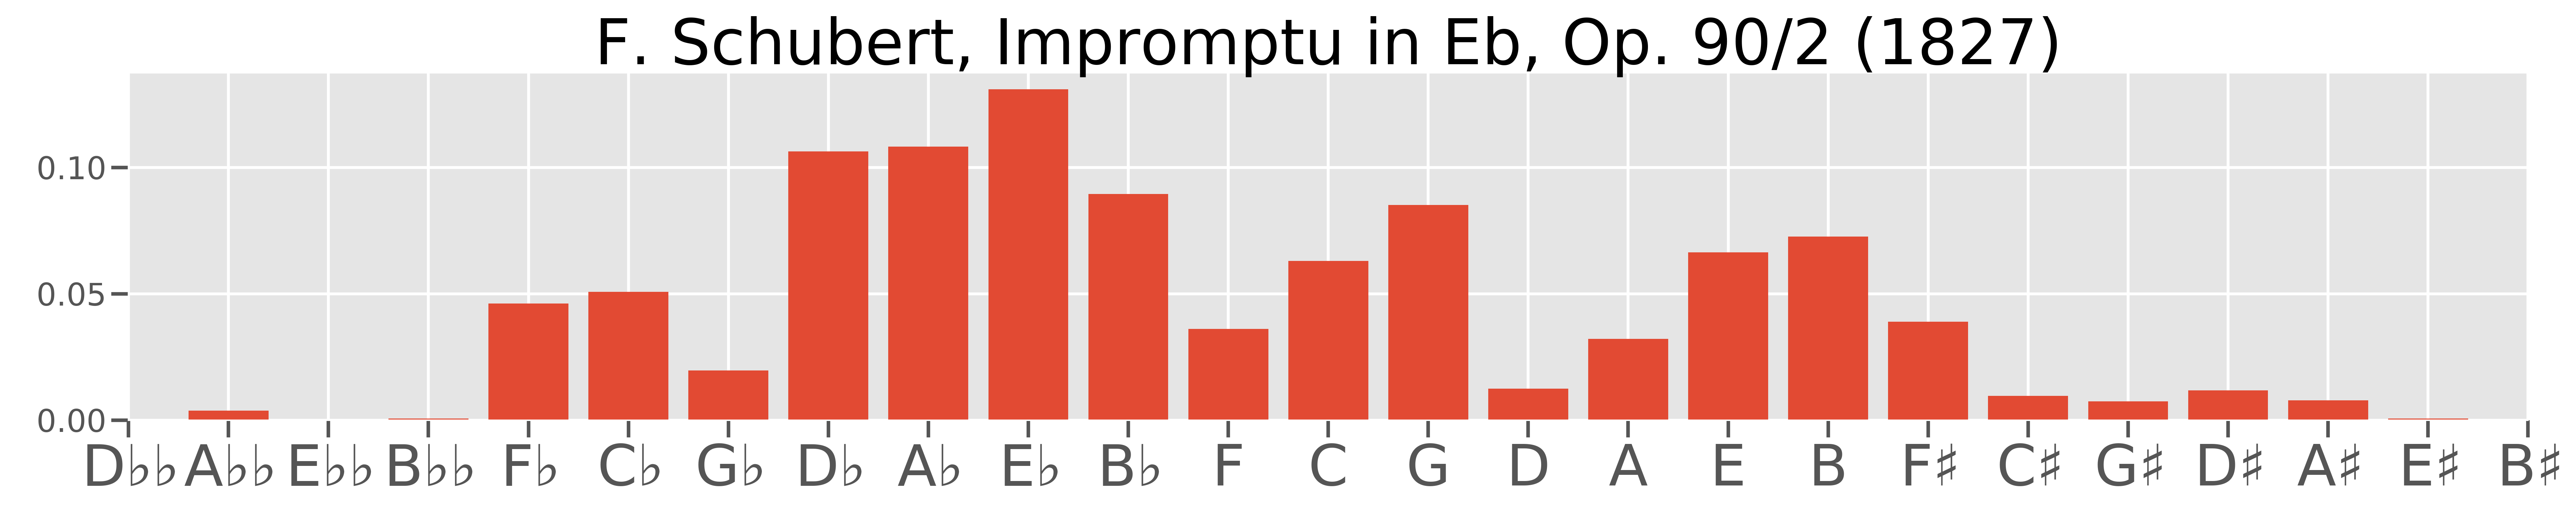
\includegraphics[width=\textwidth]{img/gmm_schubert.png}
				\end{subfigure}
			\end{figure}
      \end{block}

			\begin{block}{Conclusion}
        The often implicit or unconscious \alert{modeling assumptions about tonal spaces}
        underlying both pitch-class distributions in musical pieces and cognitive schemata
        greatly affect research outcomes. Making these assumptions explicit
        as well as incorporating music-theoretical knowledge about the
        structure of tonal spaces incorporates modeling as an integral part
        to the research on the history of tonality.
      \end{block}

			\begin{block}{References}
          \printbibliography
      \end{block}


    \end{column}

    \begin{column}{0.3\textwidth}

			\begin{block}{Model 3: Tonnetz}
        More general models of tonal space reveal further developments in tonality.
				\textbf{EXPANSION IN THIRD-DIRECTION}
				\begin{figure}
				\centering
				\begin{subfigure}{\textwidth} % width of left subfigure
					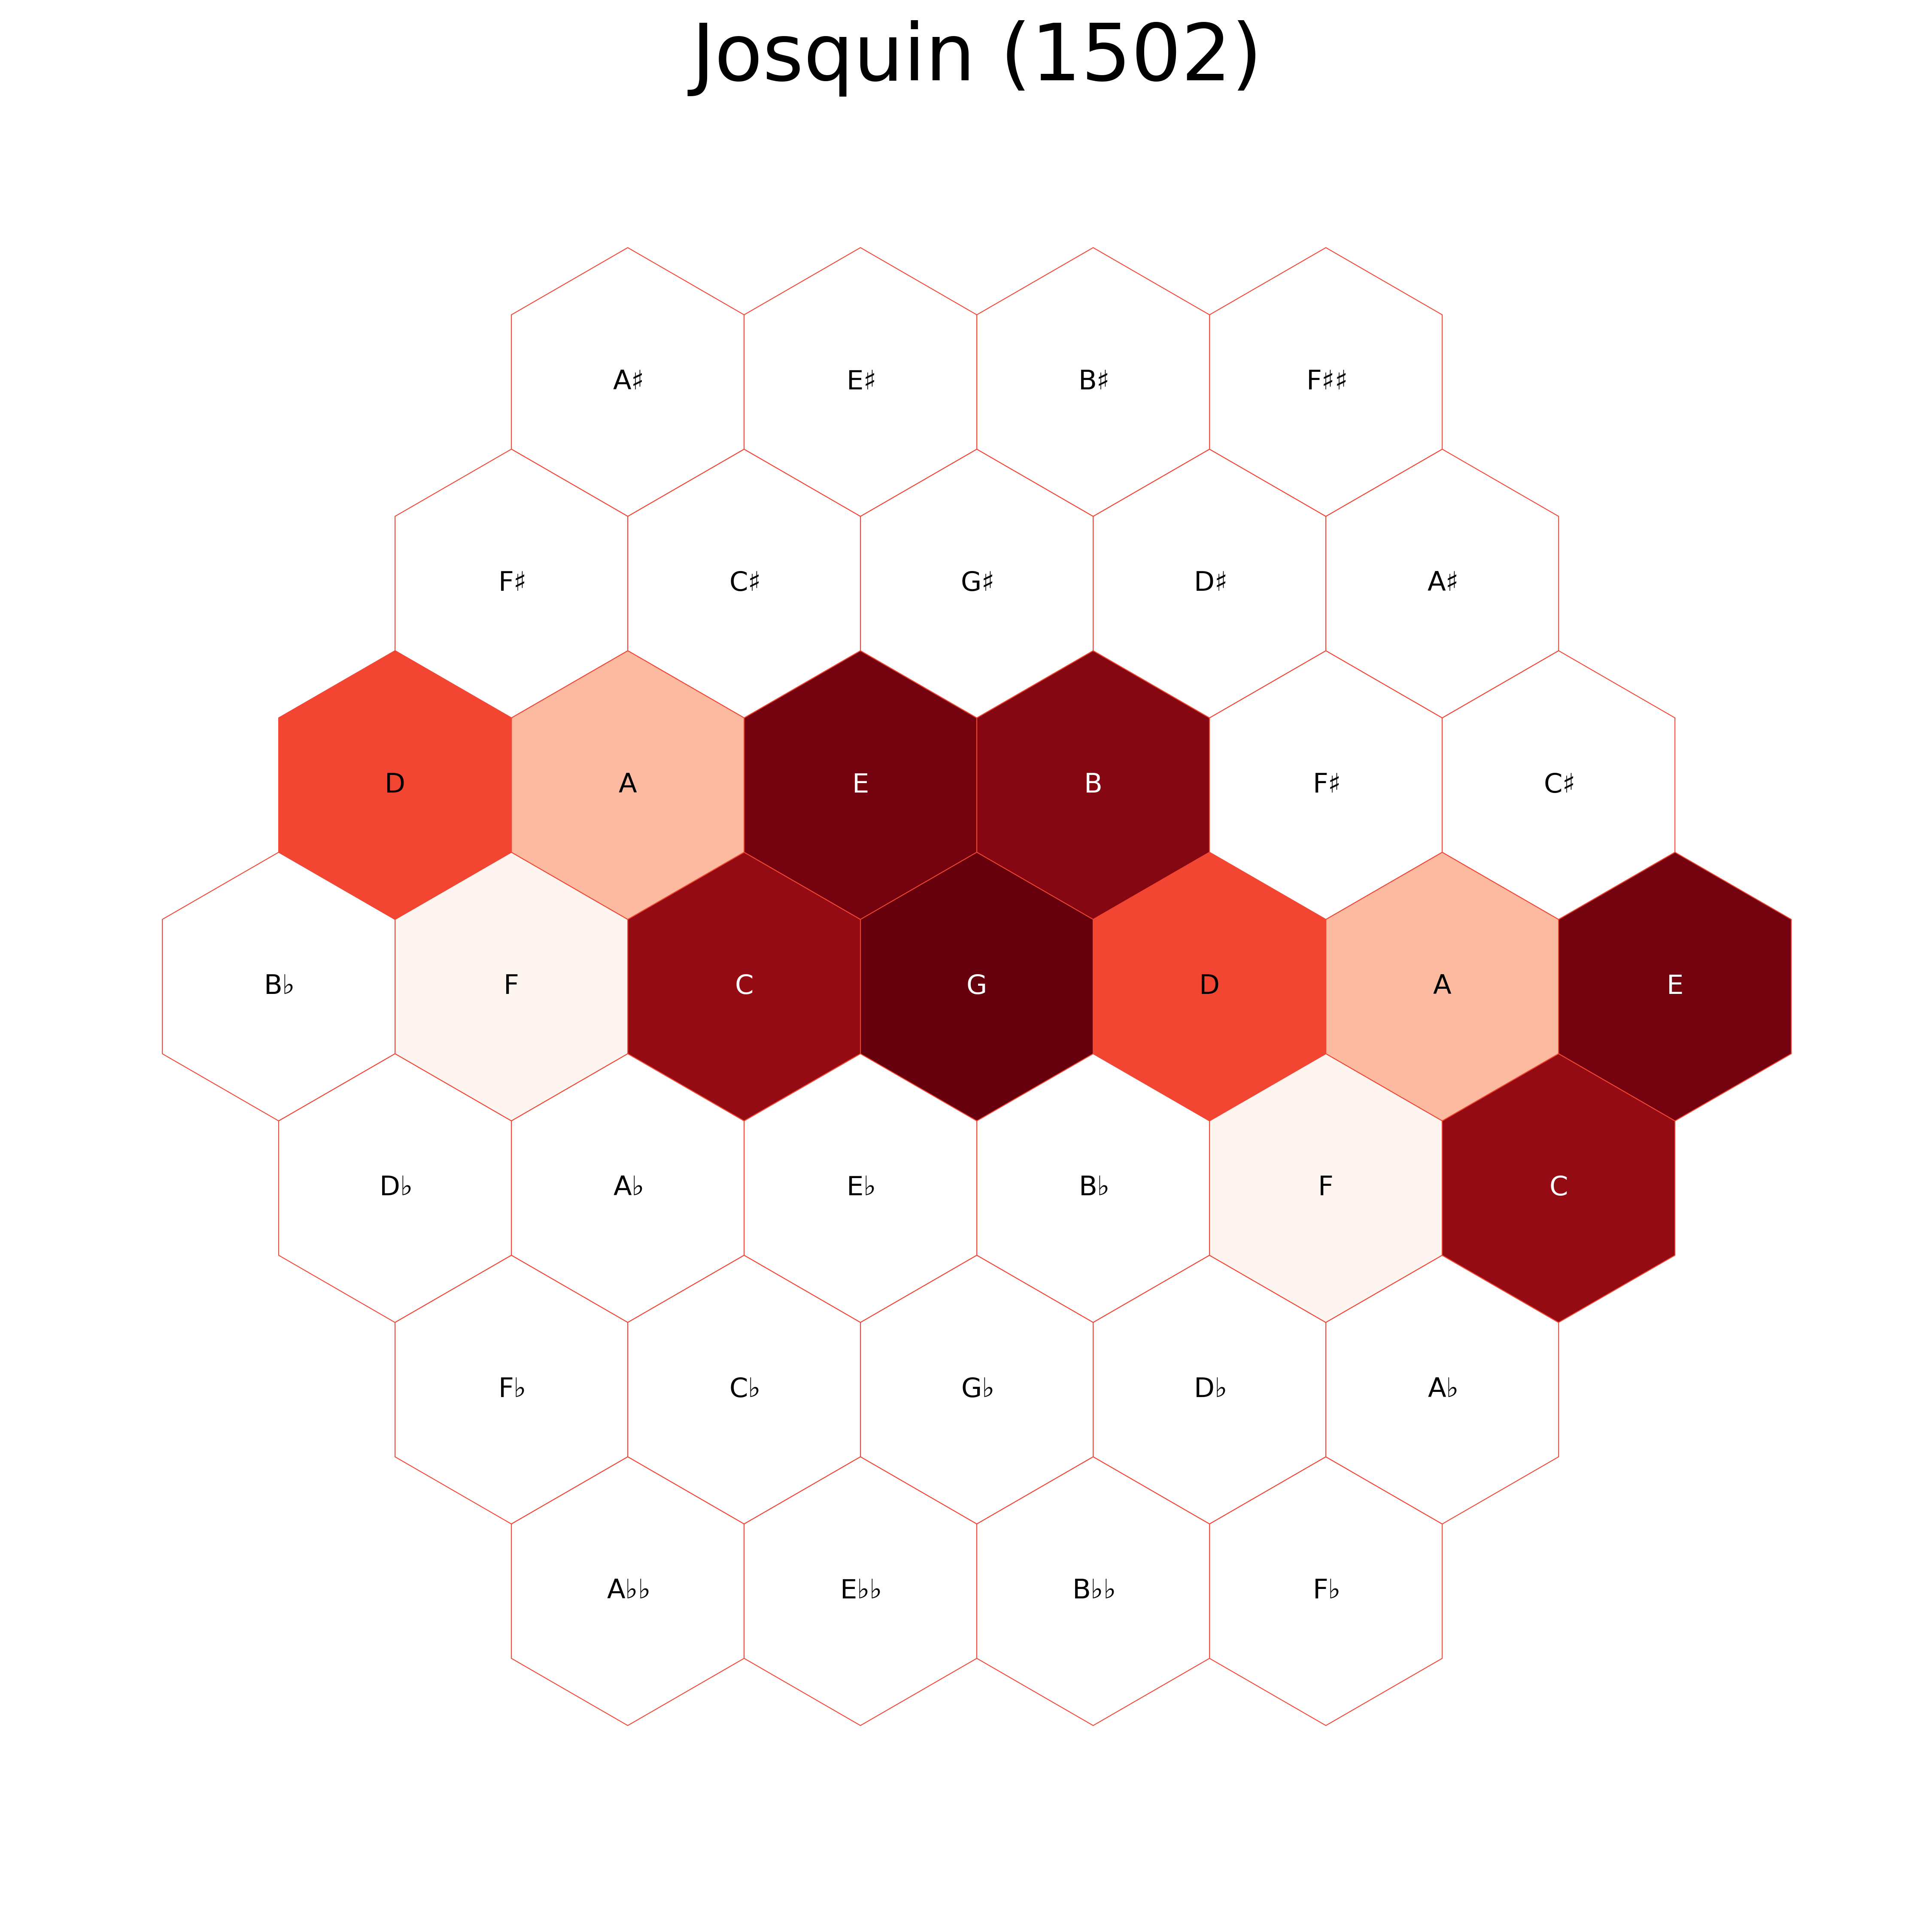
\includegraphics[width=\textwidth]{img/josquin_tonnetz.png}
				\end{subfigure}
				\begin{subfigure}{\textwidth} % width of left subfigure
					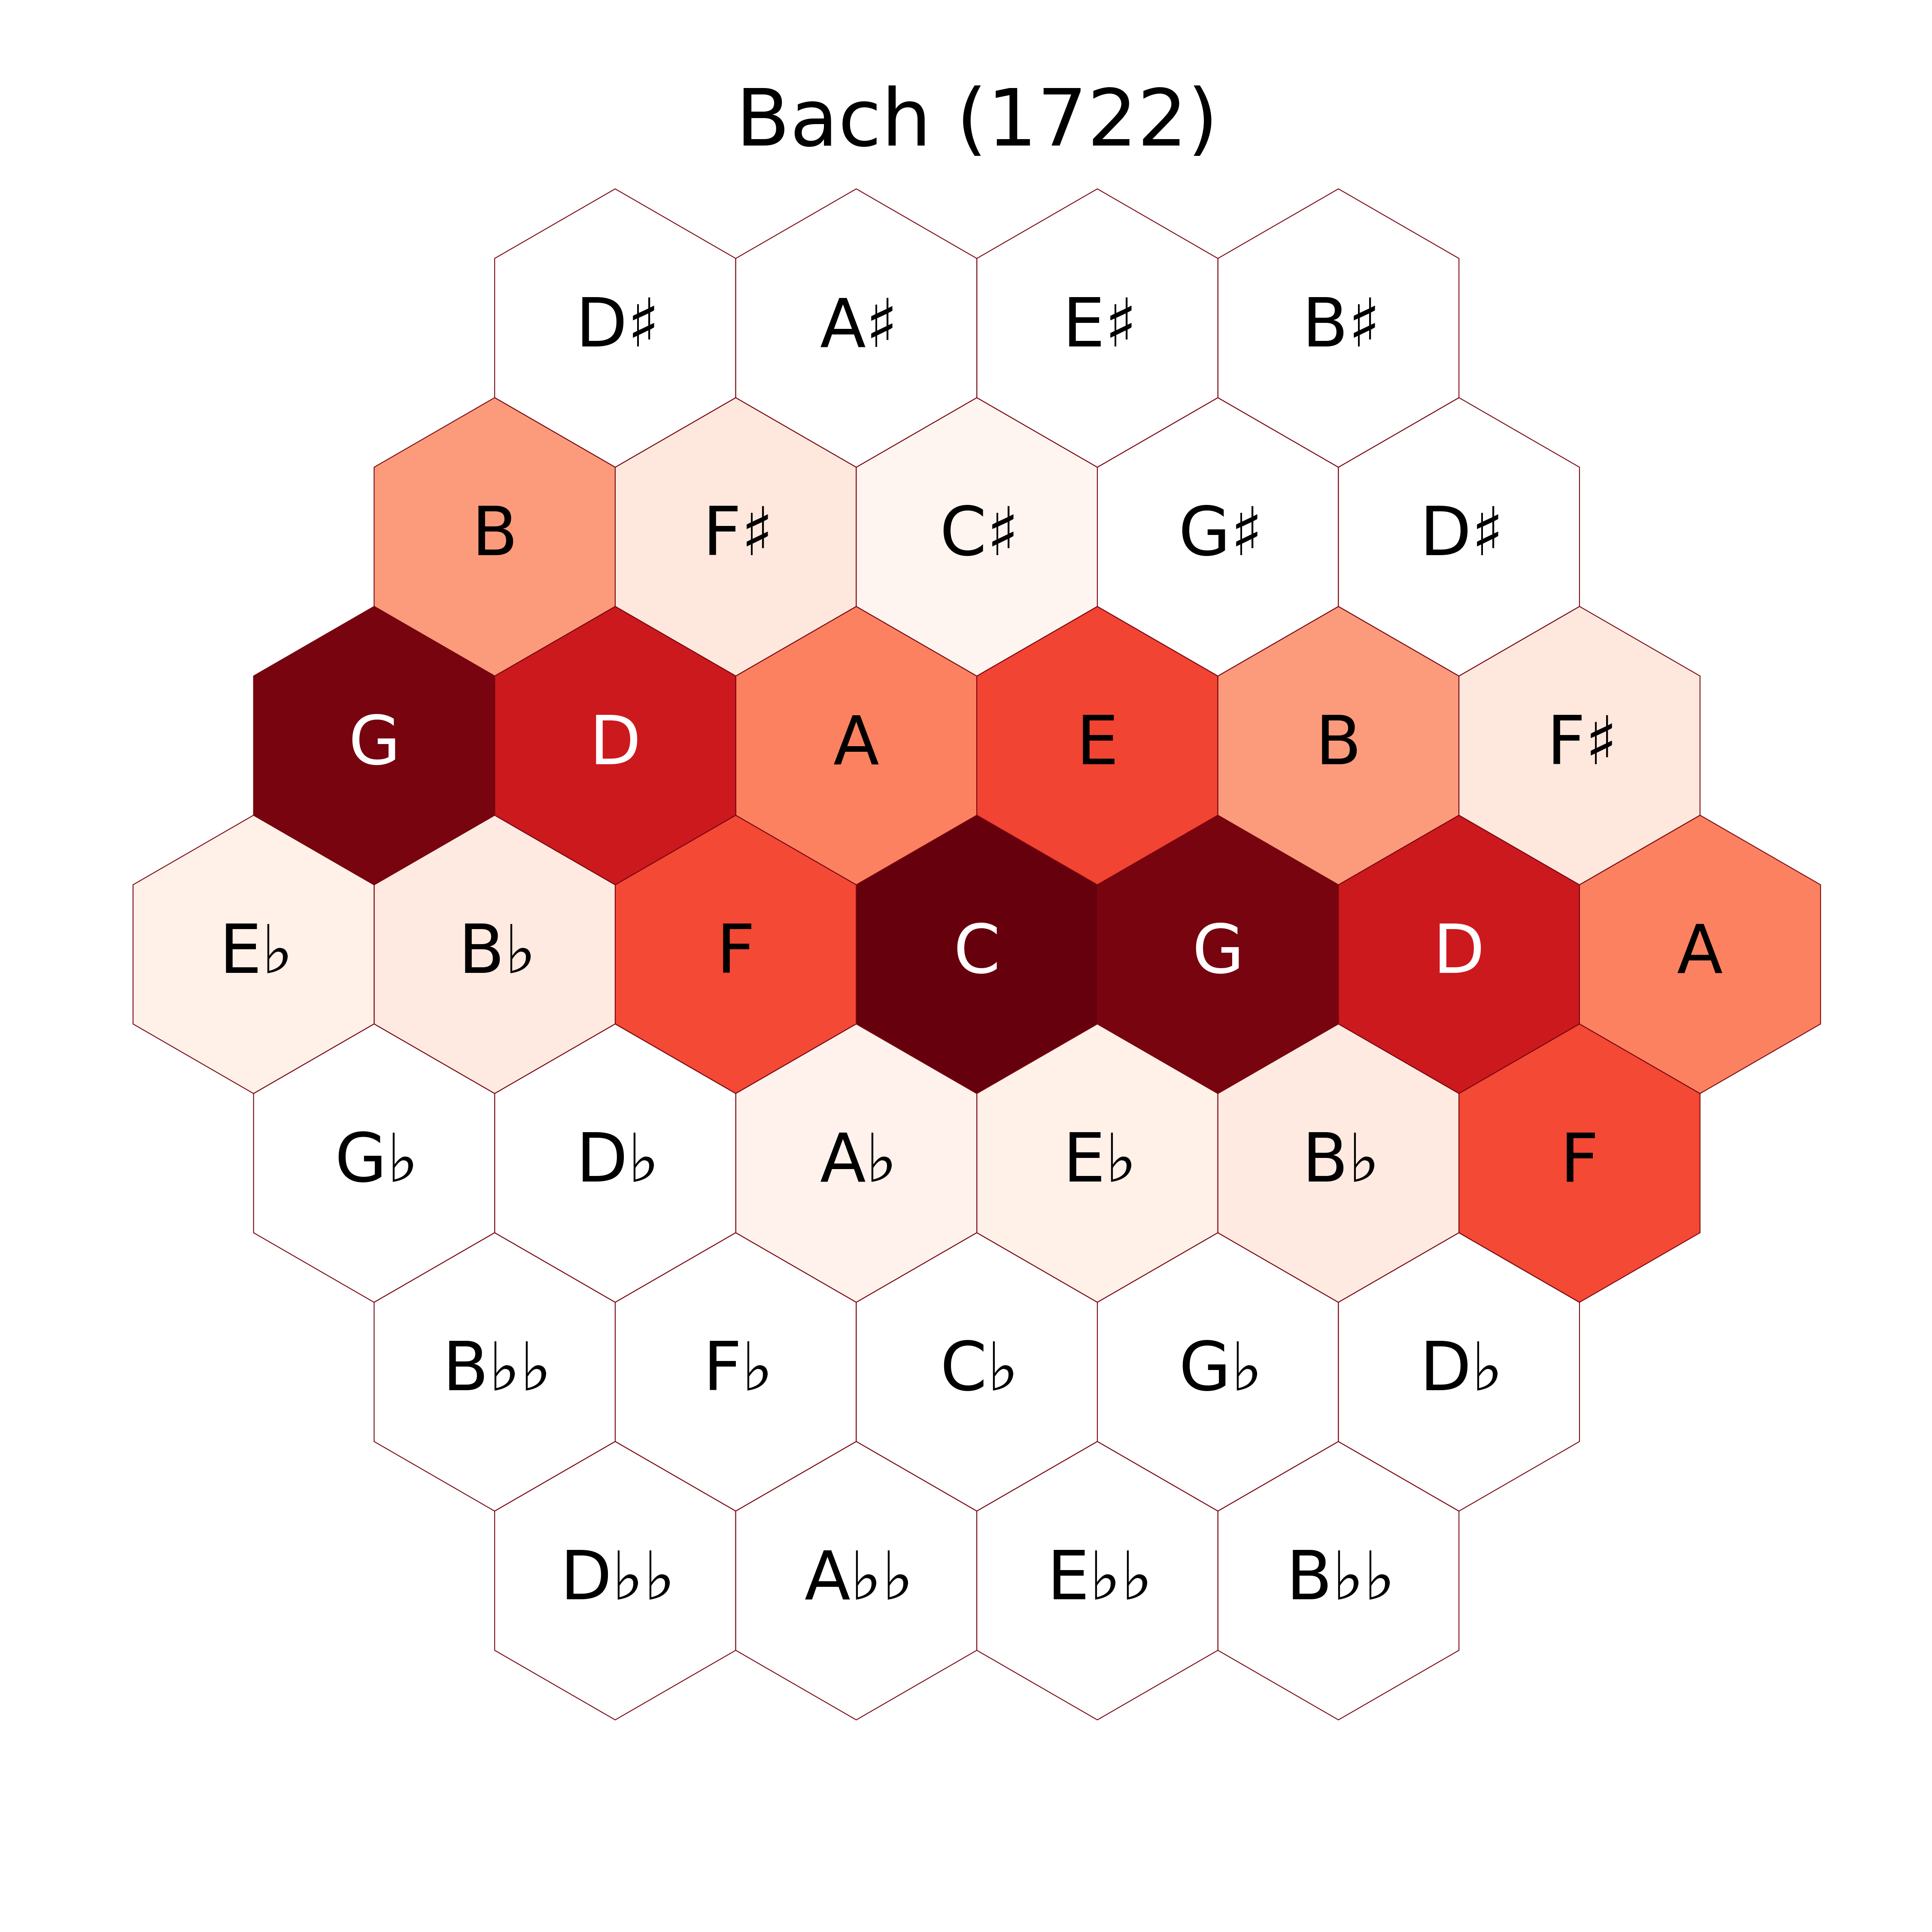
\includegraphics[width=\textwidth]{img/bach_tonnetz.png}
				\end{subfigure}
				\begin{subfigure}{\textwidth} % width of right subfigure
					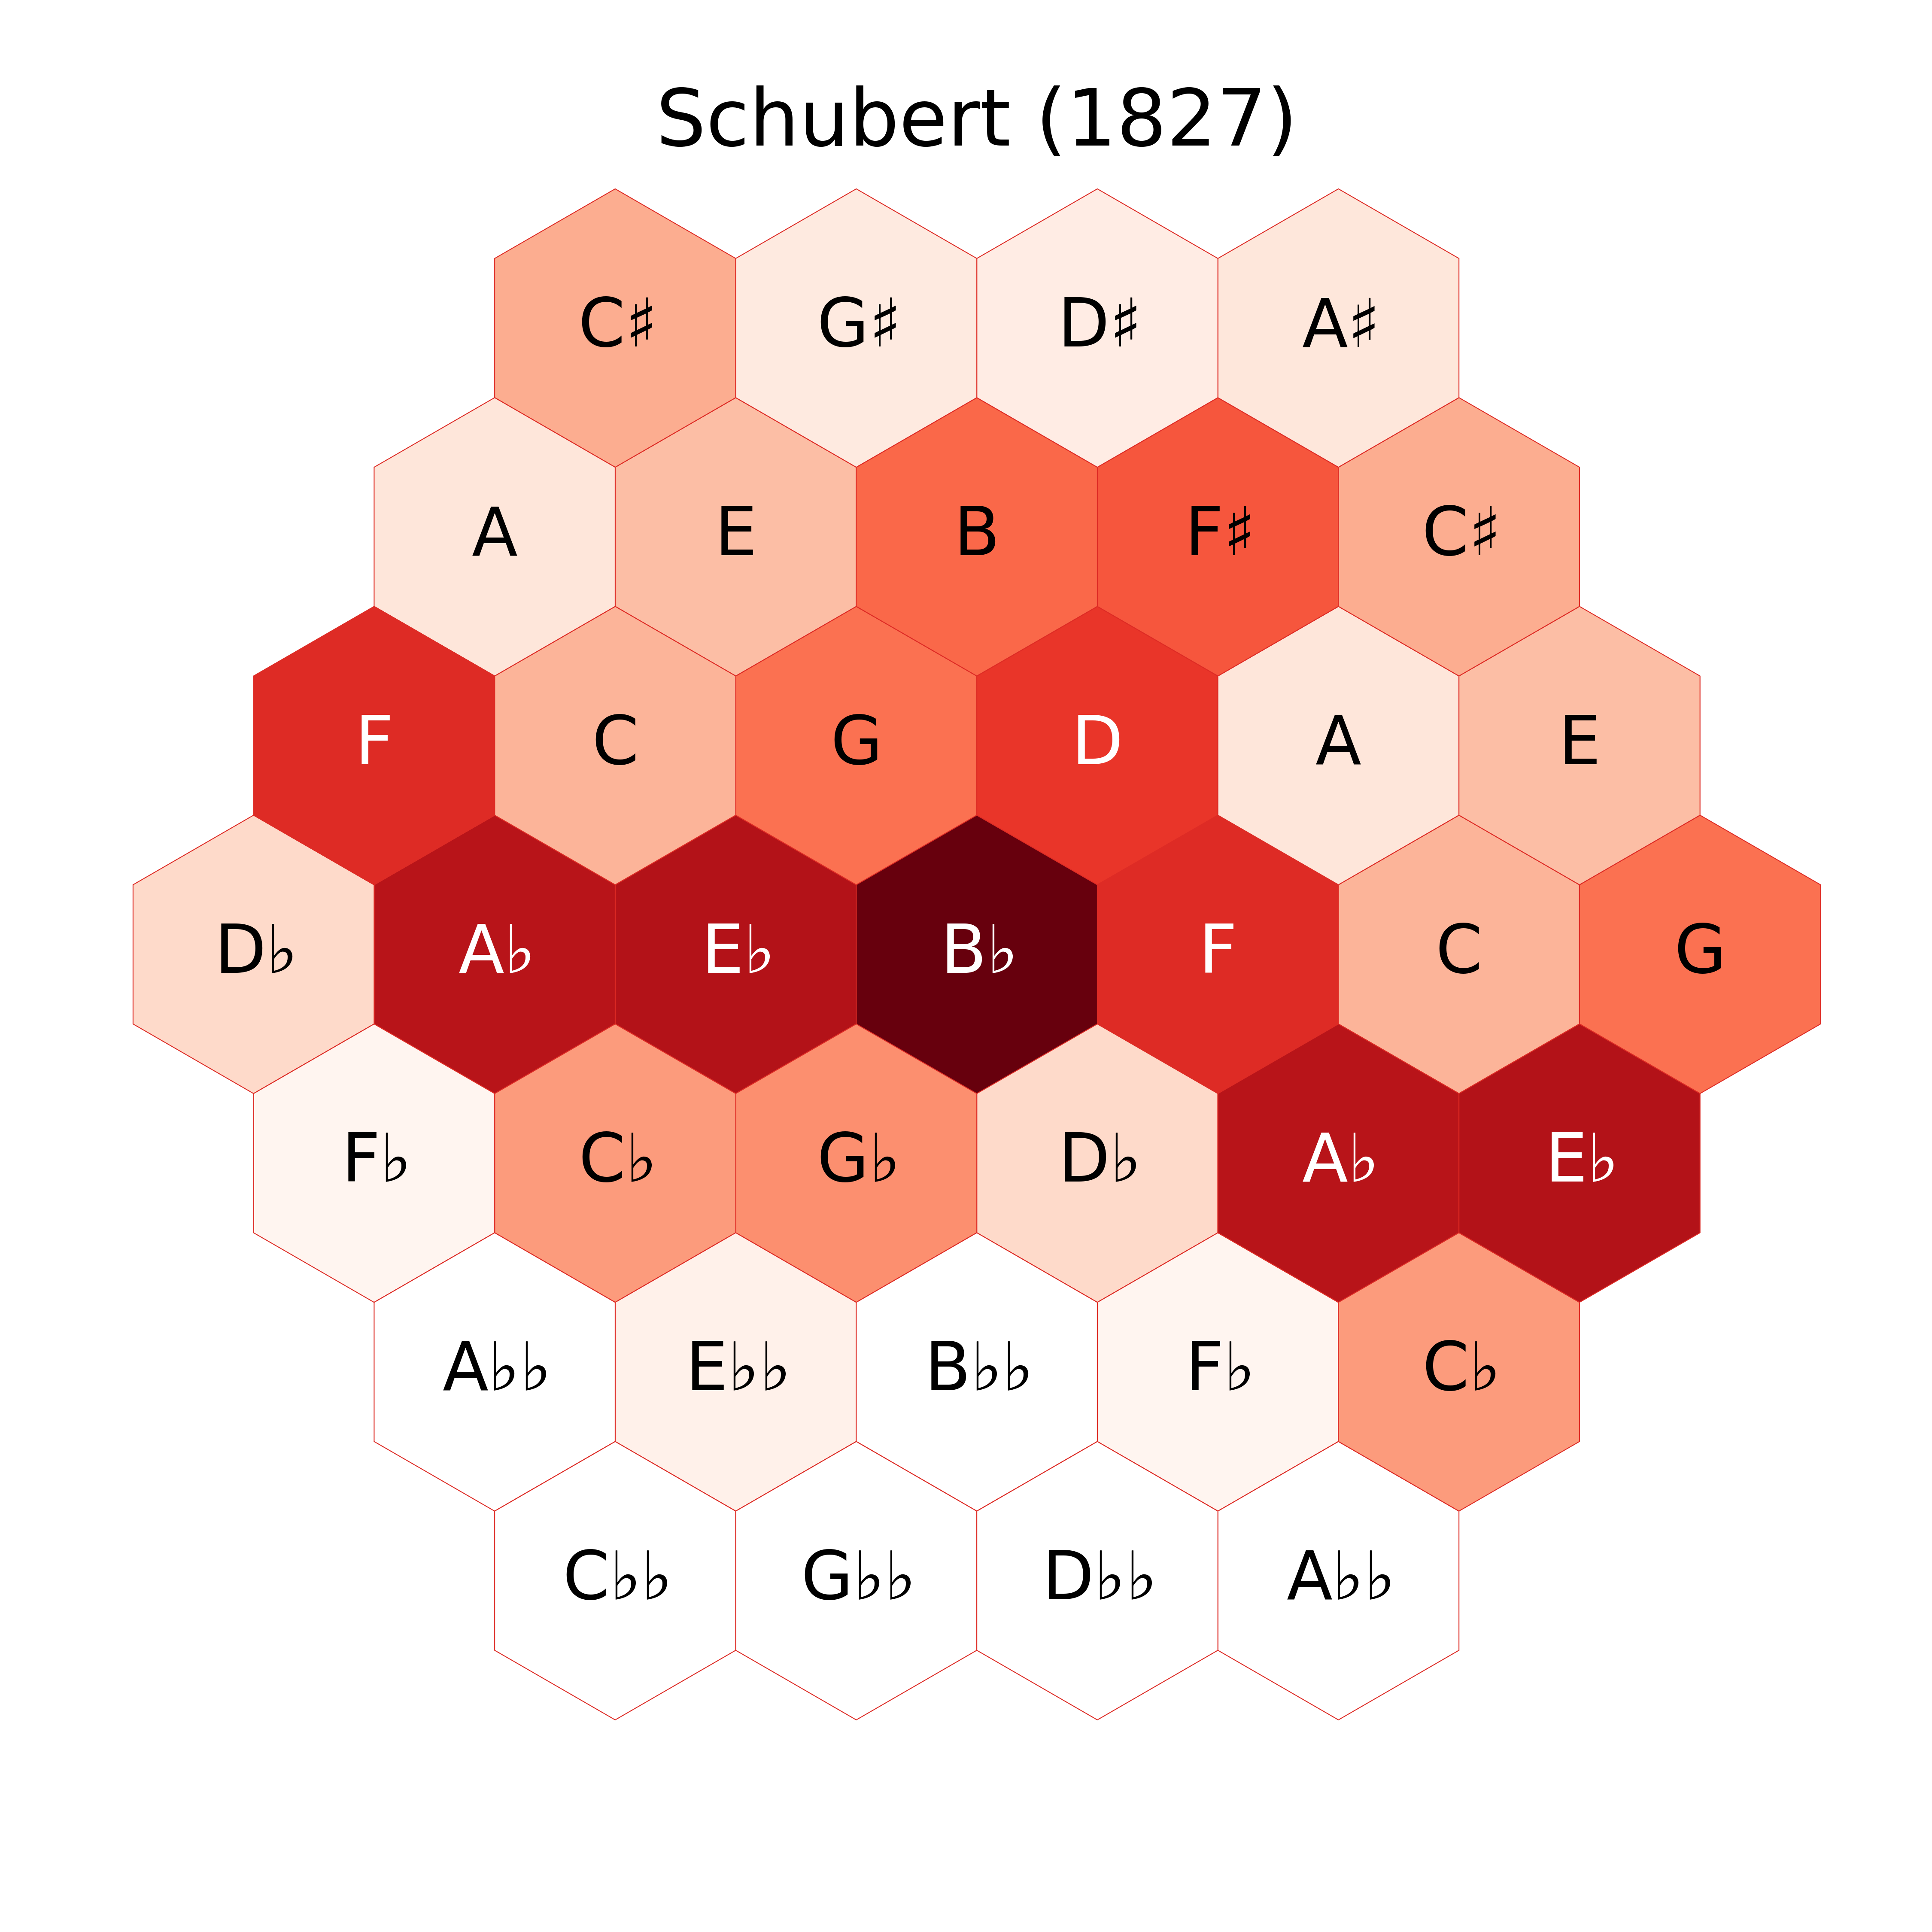
\includegraphics[width=\textwidth]{img/schubert_tonnetz.png}
				\end{subfigure}
			\end{figure}
      \end{block}

			\begin{block}{Acknowledgements \& Contact}

        \begin{wrapfigure}{l}{.5\textwidth}
					$\vcenter{\hbox{
\includegraphics[width=.5\textwidth]{img/logo_print.pdf}}}$
        \end{wrapfigure}

        \small
        This research is generously supported by the Latour Chair in Digital Musicology at EPFL.
				\normalsize
				\begin{center}
					\faicon{twitter}\;\textbf{@fabianmoss} \enspace|\enspace \faicon{envelope}\;\textbf{fabian.moss@epfl.ch}
				\end{center}
      \end{block}

    \end{column}
  \end{columns}

\end{minipage}

\begin{minipage}[t][.3\textheight][t]{\textwidth}

	\begin{columns}
		\begin{column}{.6\textwidth}
		  \begin{block}{Historical Development}

		    \begin{figure}[H]
		      \centering
					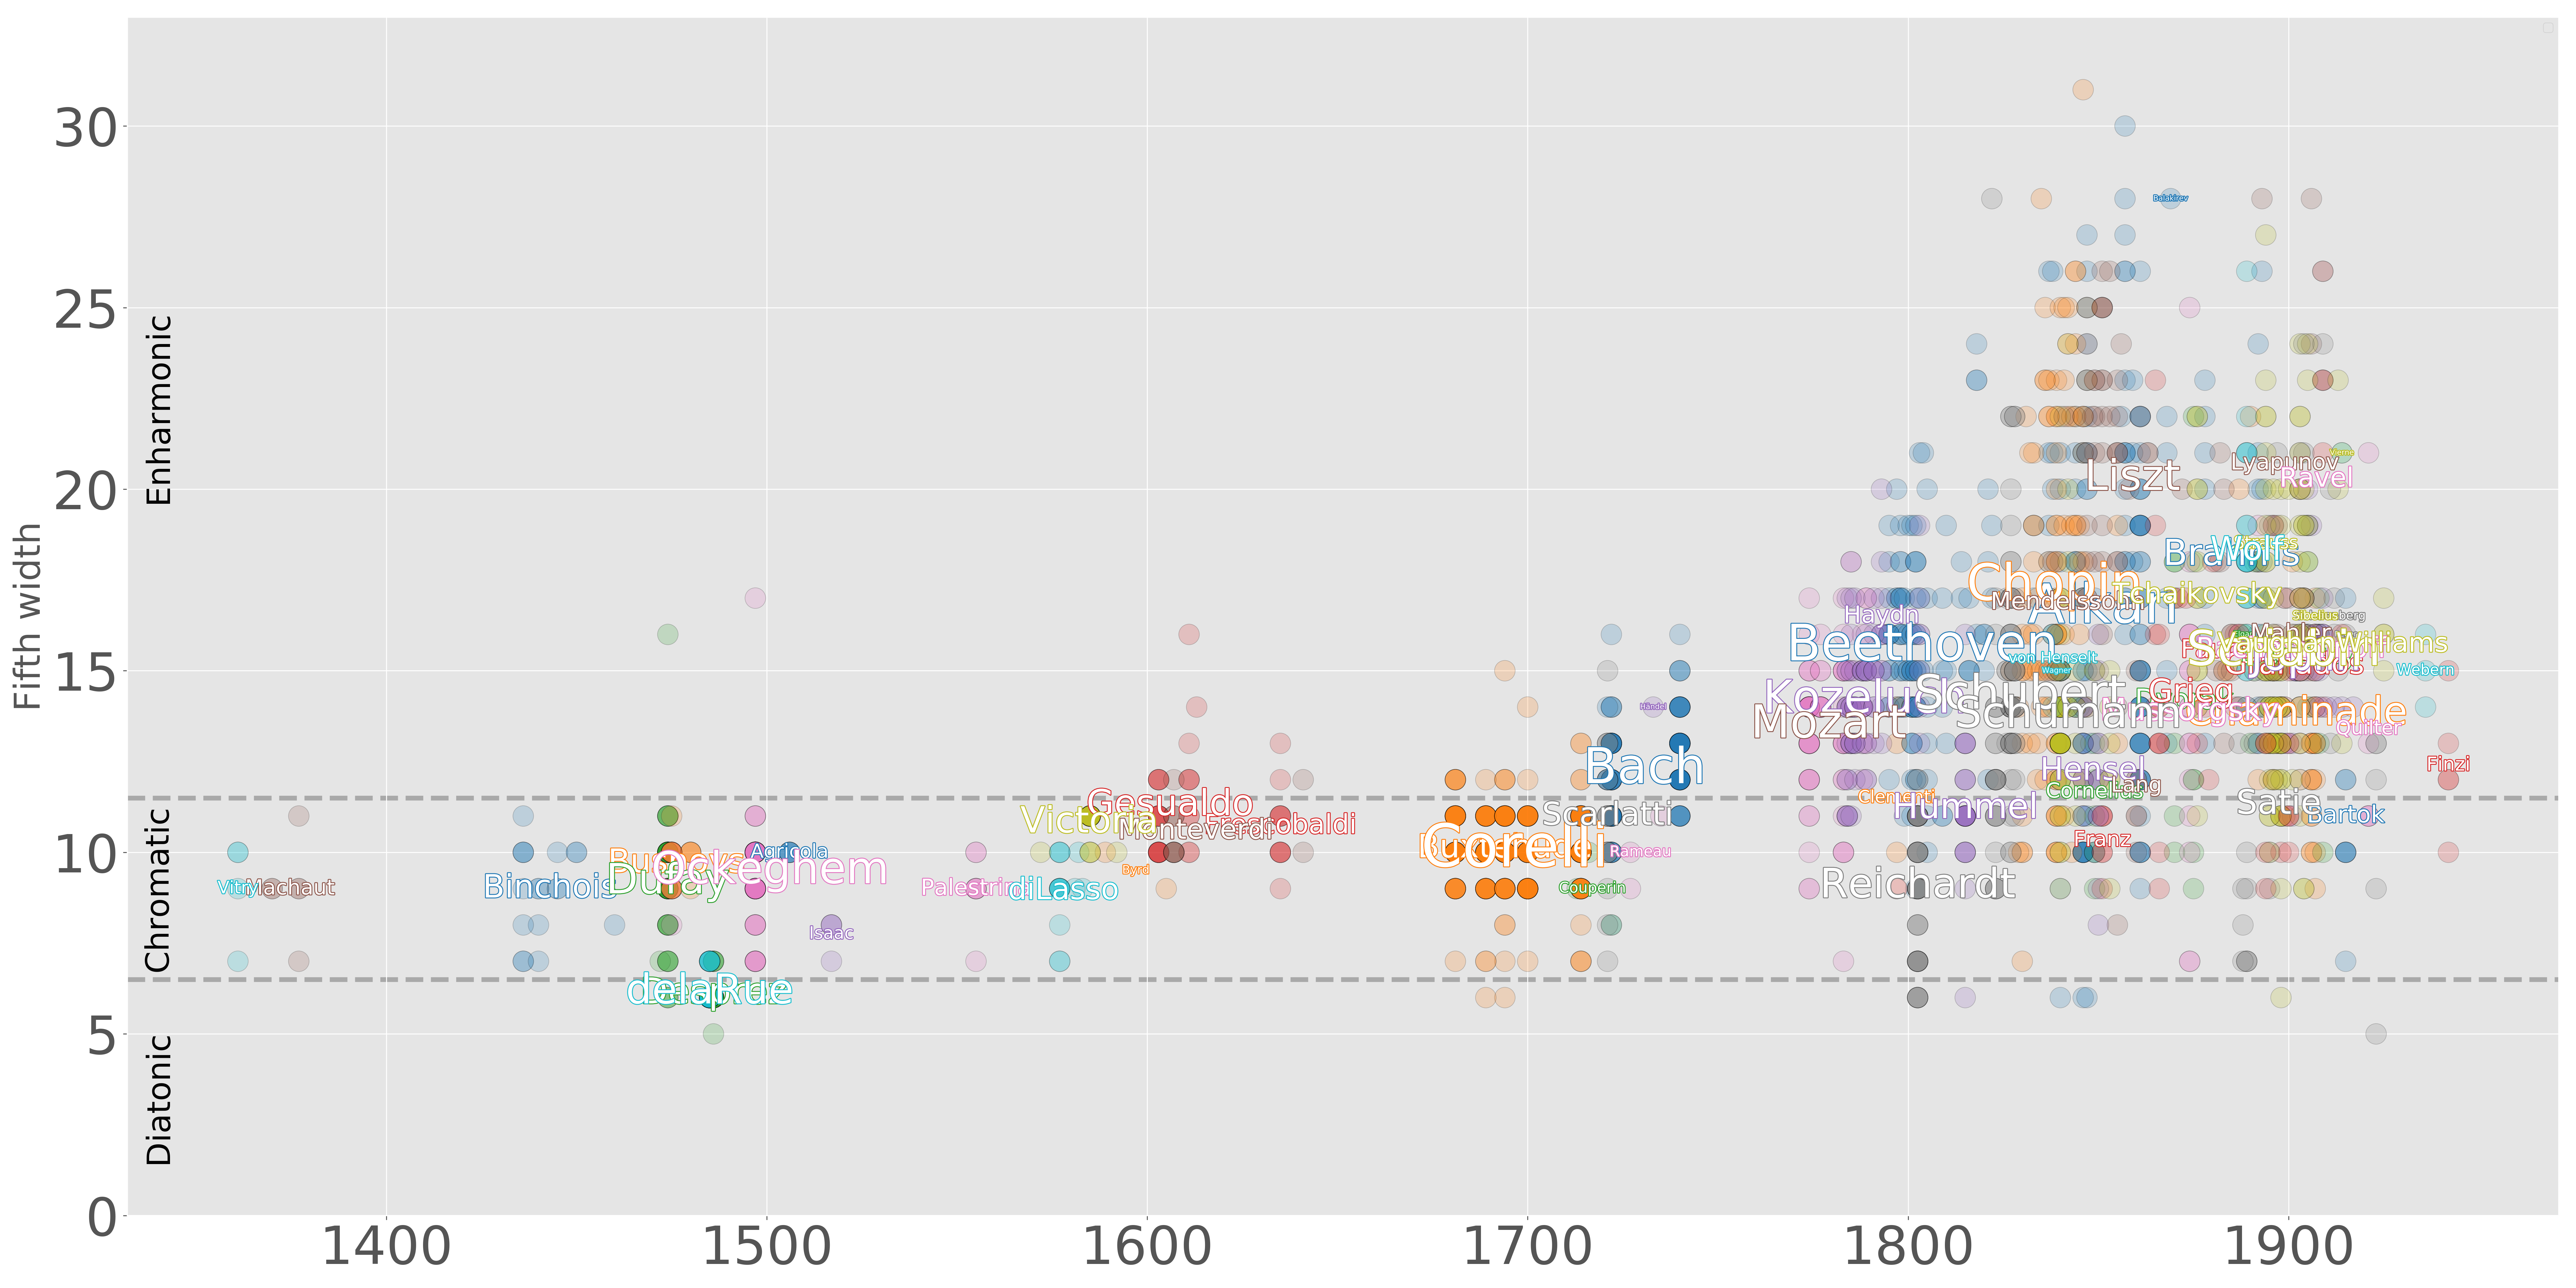
\includegraphics[width=\textwidth]{img/fifth_widths}
		      % \caption{Expansion of tonal material over the centuries.}
		      % \label{fig:history}
		    \end{figure}

		  \end{block}
		\end{column}

		\begin{column}{.3\textwidth}

		\end{column}

\end{columns}
\end{minipage}

\end{frame} % End of the enclosing frame

\end{document}
